\documentclass{article}
    % General document formatting
    \usepackage[margin=0.7in]{geometry}
    \usepackage[parfill]{parskip}
    \usepackage[utf8]{inputenc}
    
    % Related to math
    \usepackage{amsmath,amssymb,amsfonts,amsthm}
\usepackage{tikz}
\usepackage{subfigure}
\usetikzlibrary{bayesnet}

\begin{document}


\begin{figure}[ht]
\begin{center}
\begin{tabular}{cc}

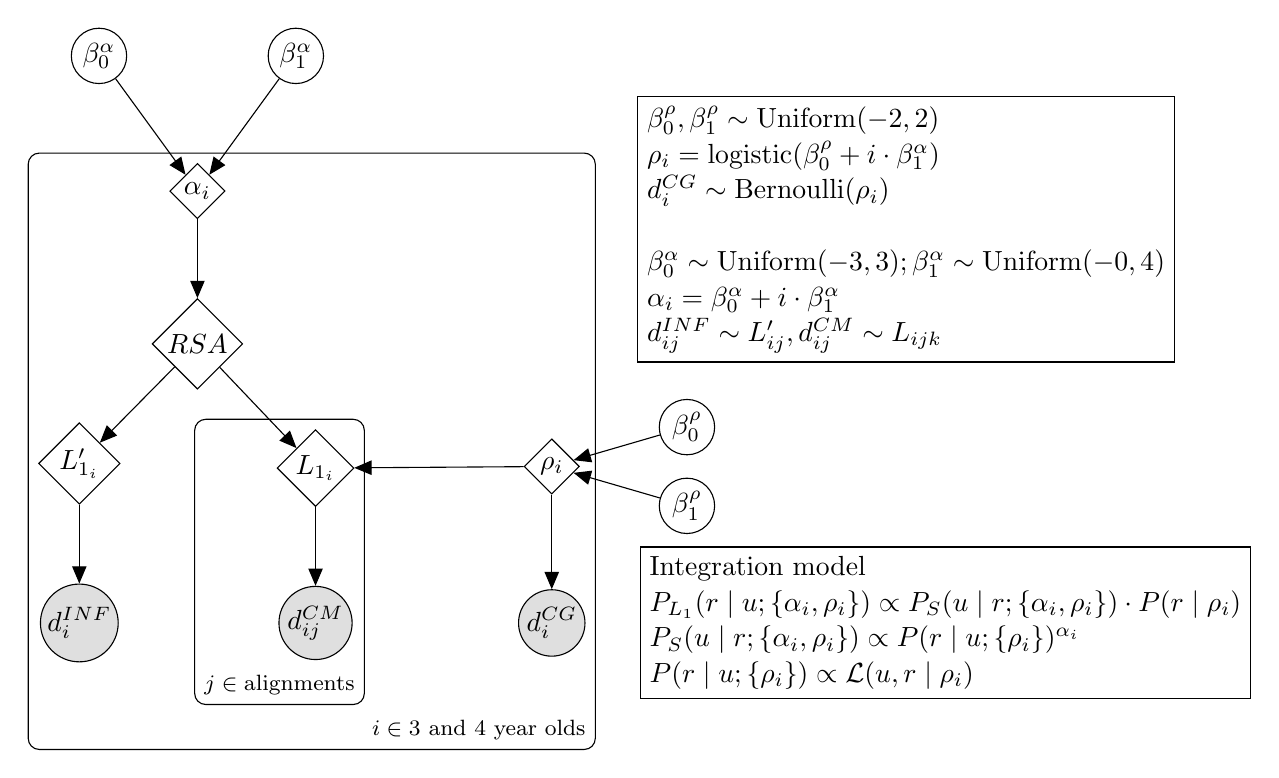
\begin{tikzpicture}
%% RSA nodes and data
\node[obs](data_comb){$d^{CM}_{ij}$};
\node[obs, xshift=-3cm, yshift=0cm](data_me){$d^{INF}_{i}$};
\node[obs, xshift=3cm,  yshift=0cm](data_cg){$d^{CG}_{i}$};

\node[det, above=of data_me](L1_me){$L'_{1_{i}}$};
\node[det, above=of data_comb](L1_comb){$L_{1_{i}}$};
\node[det, above=of L1_comb, xshift=-1.5cm, yshift=-0.5cm](RSA){$RSA$};

\edge{L1_me}{data_me};
\edge{L1_comb}{data_comb};
\edge{RSA}{L1_me};
\edge{RSA}{L1_comb};

% COMMON GROUND
\node[det, above=of data_cg, yshift=0.2cm](rho){$\rho_i$};
\node[latent, right=of rho, yshift=0.5cm](beta_rho_int){$\beta^{\rho}_0$};
\node[latent, right=of rho, yshift=-0.5cm](beta_rho_slope){$\beta^{\rho}_1$};

\edge{rho}{data_cg};
\edge{beta_rho_int}{rho};
\edge{beta_rho_slope}{rho};
\edge{rho}{L1_comb};

%% SPEAKER INFORMATIVITY

\node[det, above=of RSA, xshift=0cm](alpha){$\alpha_i$};
\node[latent, above=of alpha, xshift=-1.25cm](beta_alpha_int){$\beta^{\alpha}_0$};
\node[latent, above=of alpha, xshift=1.25cm](beta_alpha_slope){$\beta^{\alpha}_1$};

%	\edge{alpha}{L1_me};
\edge{beta_alpha_int}{alpha};
\edge{beta_alpha_slope}{alpha};
\edge{alpha}{RSA};

%% SEMANTIC KNOWLEDGE model









\

\plate{plate_condition}{(data_comb)(L1_comb)}{$j \in \text{alignments}$};


	\plate{plate_data_comb}{
	(data_comb)
	(data_cg)
	(data_me)
	(plate_condition)
	(rho)
	(alpha)
	(L1_me)
	(L1_comb)
%		(plate_items)
	}{$i \in \text{3 and 4 year olds}$}



\node[draw, align=left, execute at begin node=\setlength{\baselineskip}{3ex}] at (7.5,5) { 
$\beta^\rho_0 ,\beta^\rho_1 \sim \text{Uniform}(-2,2)$ \\
 $\rho_i = \text{logistic}(\beta^\rho_0  + i \cdot \beta^\alpha_1)$ \\
 $d^{CG}_{i} \sim \text{Bernoulli}(\rho_i)$ \\
 \\
$\beta^\alpha_0 \sim \text{Uniform}(-3,3); \beta^\alpha_1 \sim \text{Uniform}(-0,4)$ \\
 $\alpha_i = \beta^\alpha_0  + i \cdot \beta^\alpha_1$ \\
 $d^{INF}_{ij} \sim L'_{ij},  d^{CM}_{ij} \sim L_{ijk}$
};

\node[draw, align=left, execute at begin node=\setlength{\baselineskip}{3ex}] at (8,0) {Integration model\\ 
$P_{L_{1}}(r \mid u; \{\alpha_i,\rho_i\})\propto P_{S}(u \mid r; \{\alpha_i,\rho_i\}) \cdot P(r \mid \rho_i) $\\ 
$P_{S}(u \mid r; \{\alpha_i, \rho_i\})\propto P(r \mid u; \{\rho_i\}) ^{\alpha_i} $\\
$P(r \mid u; \{\rho_i\}) \propto \mathcal{L}(u, r \mid \rho_i)$
};


\end{tikzpicture}


\\
\\
\\
\\
\\

%S2 represents the RSA speaker model defined by Eq. 1, which is used to predict the production responses dprod of each participant i, for each state s (number of hearts), for each utterance w, in each goal condition g. The RSA speaker model takes as input the literal meaning variables θ, which additionally are used to predict the literal meaning judgments dlit assuming a Bernoulli linking function. Additionally, the RSA model takes the speaker’s goal weights ω and intended presentational goal weight φ, which are inferred separately for each goal condition g. Finally, the RSA model uses two global free parameters: the cost of negation c and the speaker’s rationality parameter α.

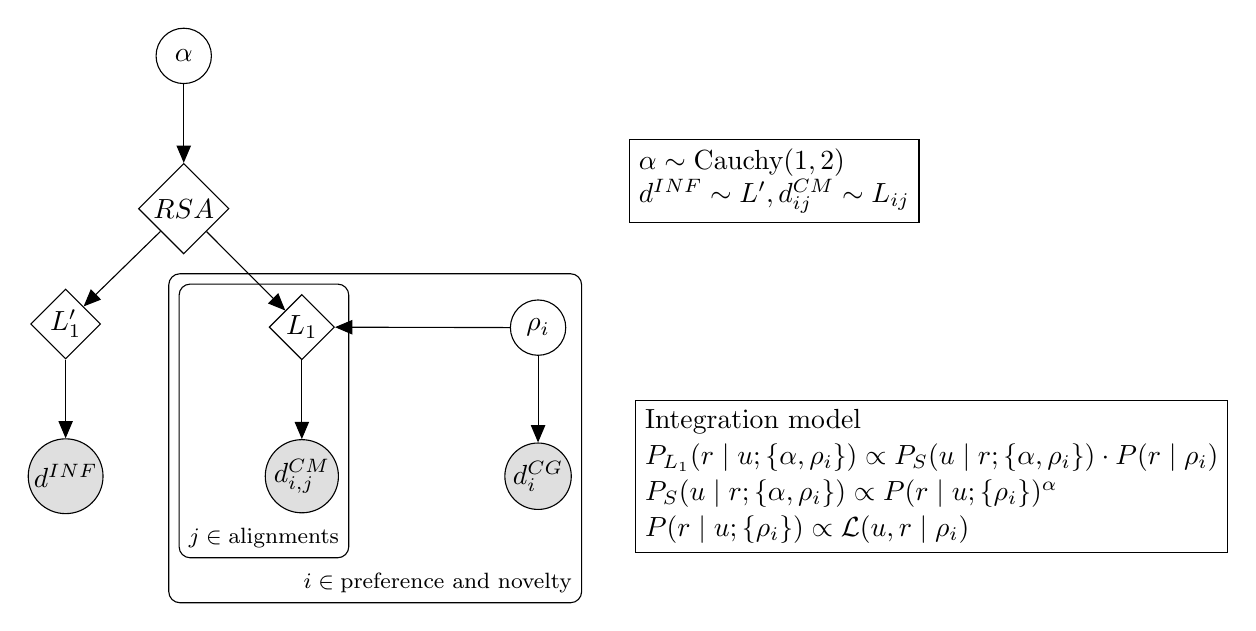
\begin{tikzpicture}
%% RSA nodes and data
\node[obs](data_comb){$d^{CM}_{i,j}$};
\node[obs, xshift=-3cm, yshift=0cm](data_me){$d^{INF}$};
\node[obs, xshift=3cm,  yshift=0cm](data_cg){$d^{CG}_{i}$};

\node[det, above=of data_me](L1_me){$L'_{1}$};
\node[det, above=of data_comb](L1_comb){$L_{1}$};
\node[det, above=of L1_comb, xshift=-1.5cm, yshift=-0.5cm](RSA){$RSA$};

\edge{L1_me}{data_me};
\edge{L1_comb}{data_comb};
\edge{RSA}{L1_me};
\edge{RSA}{L1_comb};

% COMMON GROUND
\node[latent, above=of data_cg, yshift=0.1cm](rho){$\rho_{i}$};

\edge{rho}{data_cg};
\edge{rho}{L1_comb};

%% SPEAKER INFORMATIVITY

\node[latent, above=of RSA, xshift=0cm](alpha){$\alpha$};

%	\edge{alpha}{L1_me};
\edge{alpha}{RSA};

\

\plate{plate_condition}{(data_comb)(L1_comb)}{$j \in \text{alignments}$};


	\plate{plate_data_comb}{
	(data_comb)
	(data_cg)
	(plate_condition)
	(rho)
%		(plate_items)
	}{$i \in \text{preference and novelty}$}



\node[draw, align=left, execute at begin node=\setlength{\baselineskip}{2ex}] at (6,3.75) { 
$\alpha \sim \text{Cauchy}(1,2)$ \\
$d^{INF} \sim L',  d^{CM}_{ij} \sim L_{ij}$
};

\node[draw, align=left, execute at begin node=\setlength{\baselineskip}{3ex}] at (8,0) {Integration model\\ 
$P_{L_{1}}(r \mid u; \{\alpha,\rho_i\})\propto P_{S}(u \mid r; \{\alpha, \rho_i\}) \cdot P(r \mid \rho_i) $\\ 
$P_{S}(u \mid r; \{\alpha, \rho_i\})\propto P(r \mid u; \{\rho_i\}) ^{\alpha} $\\
$P(r \mid u; \{\rho_i\}) \propto \mathcal{L}(u, r \mid \rho_i)$
};


\end{tikzpicture}

  \end{tabular}
  \end{center}
  \label{fig:bayesnet}
\end{figure}



\end{document}

